\hypertarget{section-runtime-view}{%
\section{Runtime View}\label{section-runtime-view}}
In this section we wanted to describe our two most important use-cases in more detail to allow for better understanding.

\subsection{Opening \& starting a lobby}
In order to start an escape-room and allow students to join a few steps have to be taken. The lector first needs to authenticate via our auth. provider after which a lobby can be opened. After opening a lobby students can join via the provided id, which in this case would be 1. When joining a lobby the students get a websocket in response for all subsequent communication from the server to the client. As soon as the lector starts the lobby, the Player API gets informed of this action as it's responsible for notifying all students participating.
\begin{figure}[h!]
    \centering
    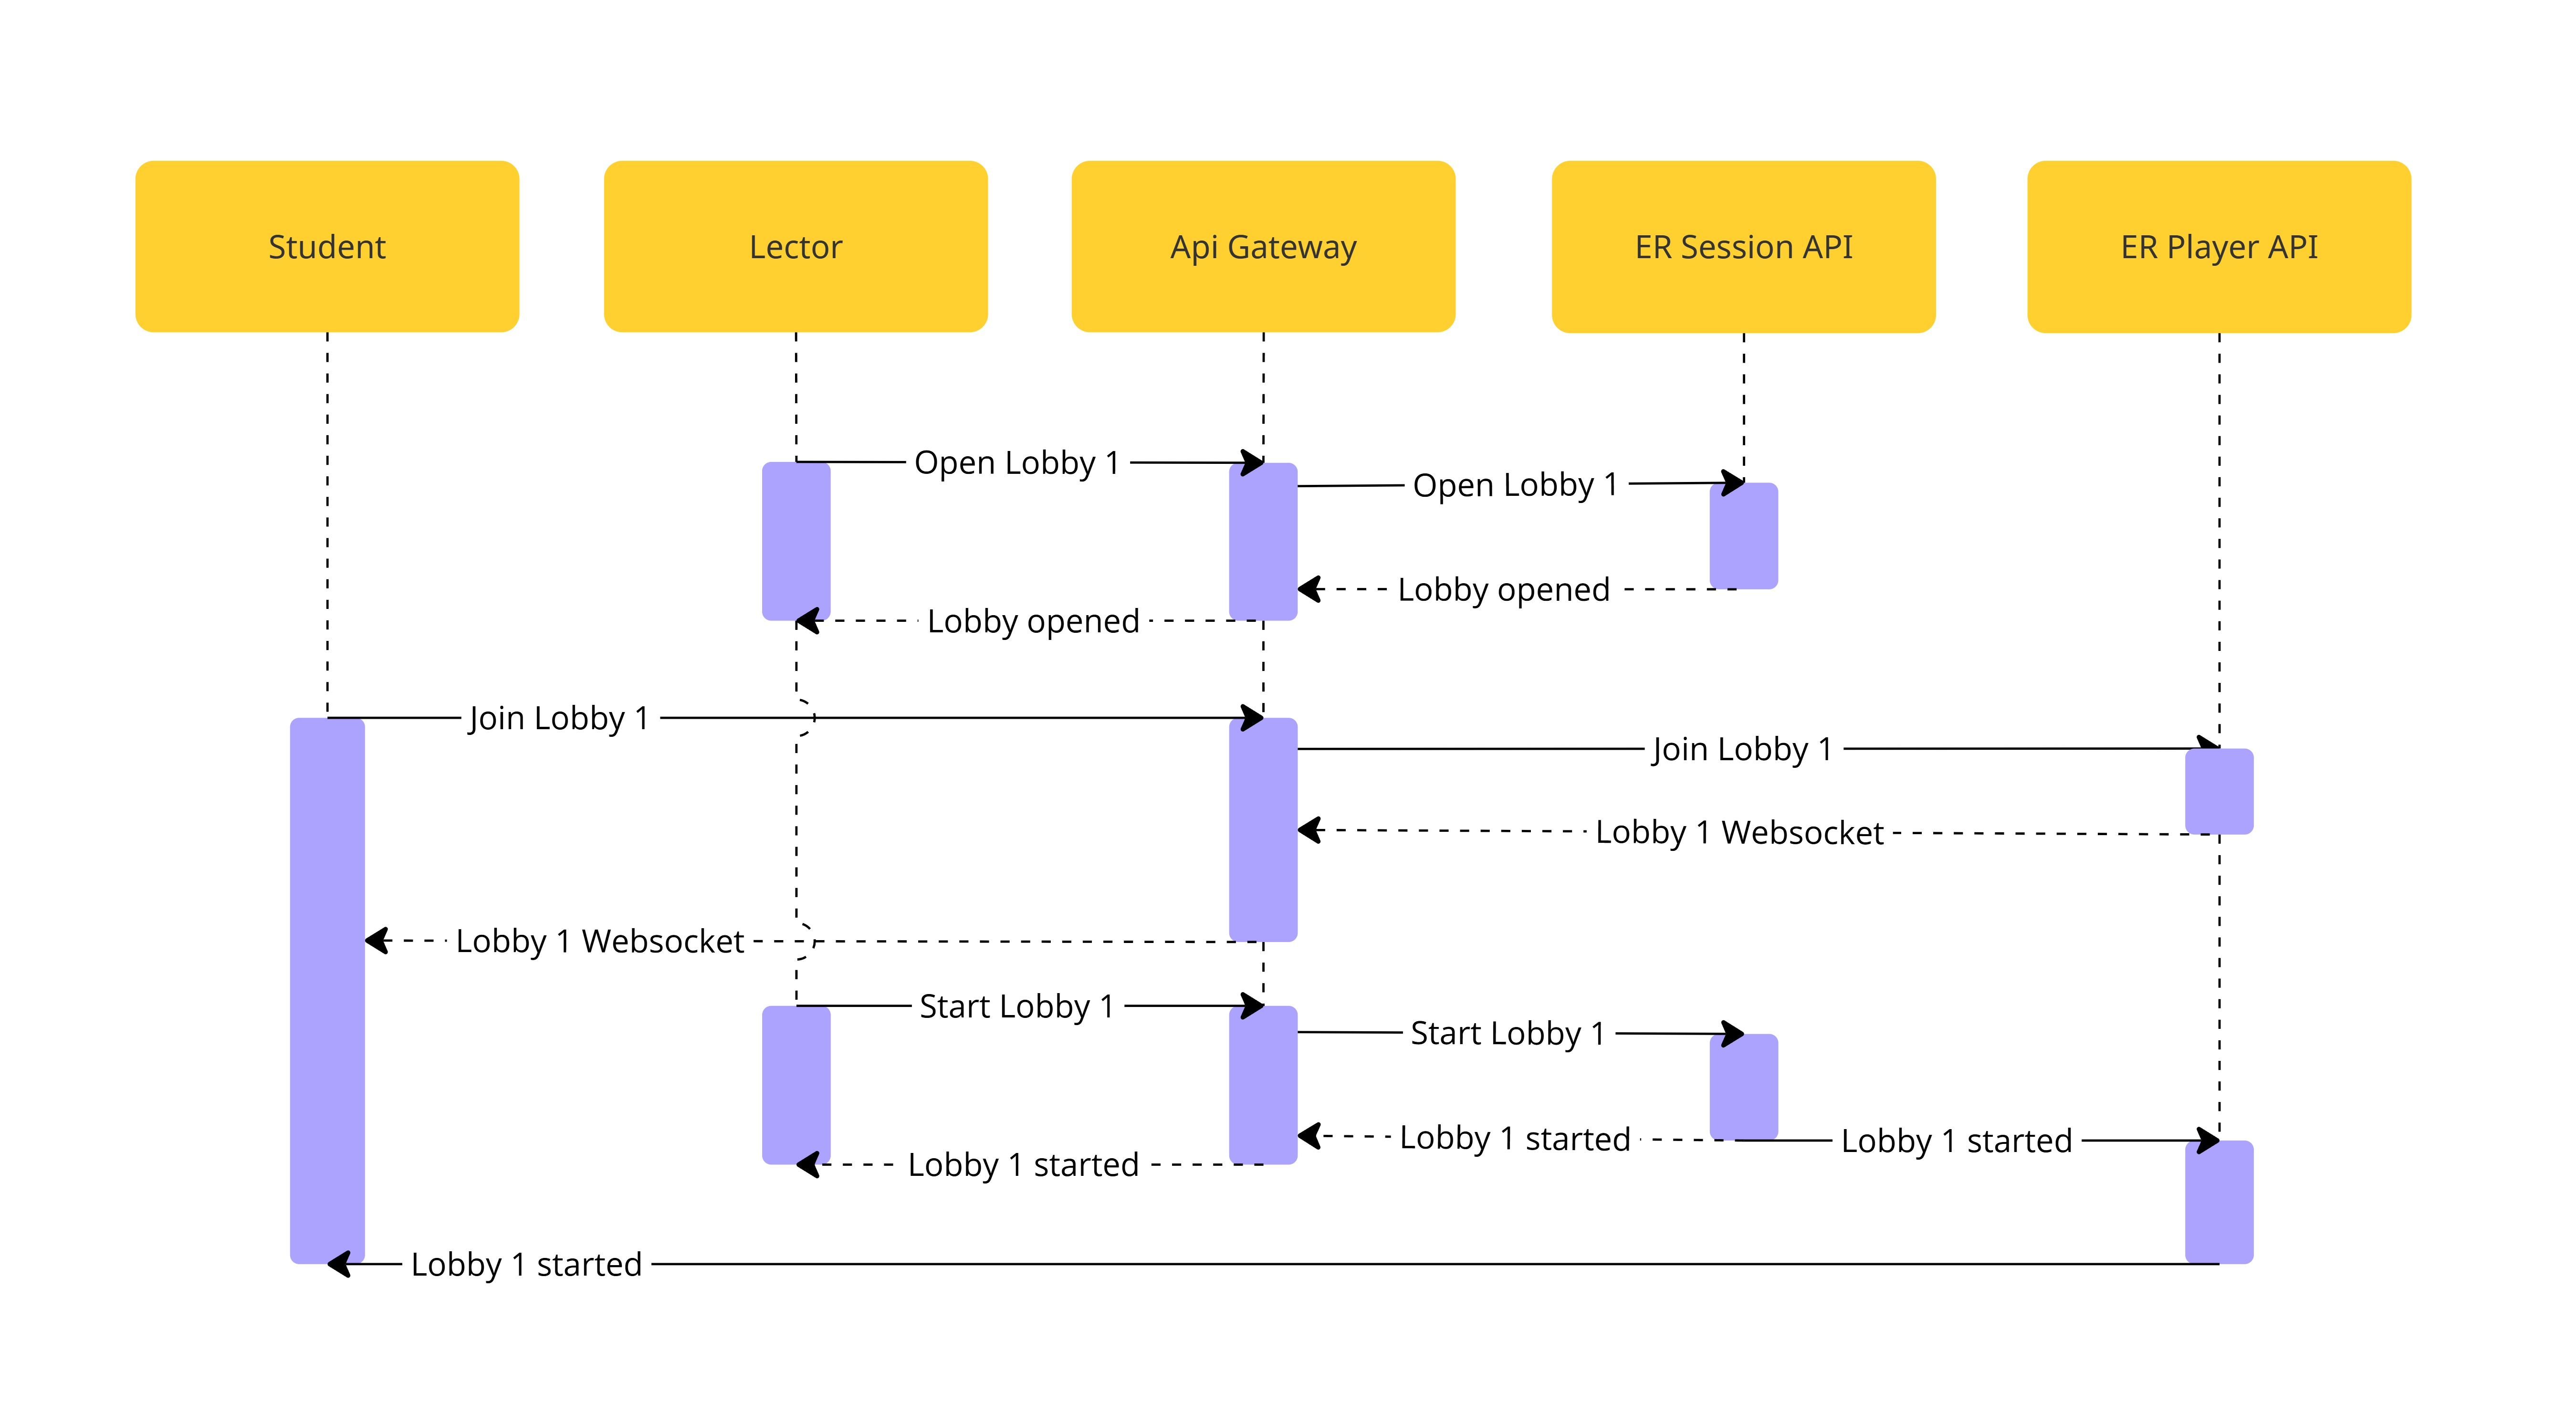
\includegraphics[width=1\linewidth]{images/Sequence Diagrams/SEP1 - EscapeDOOM - Open Lobby - Start Lobby.jpg}
    \caption{Opening and starting a lobby with a student join}
    \label{fig:sequenceDiag:openAndStart}
\end{figure}

\newpage

\subsection{Sending riddle solution}

After an escape-room has been and all students joined a session, the main 'mechanic' of the escape-room is to accept code snippets and run them to validate the solution.

In order to do this, students get the current stage of the session pushed to them. When they now choose to submit the a solution, it will get sent to the Player API which will forward the code to the executor. The executor will run the code and return a result depending on the success or failure of the submitted code. Afterwards the response gets returned to the Students via the Player API. In the case that the solution was correct, the student is given the option to continue to the next stage or stay longer if they choose to. When the request to go to the next stage is submitted, the Player API pushes the next stage to the client, at which point this process can be repreated until the escape room is done. \\
Additionally Students can choose to view the leaderboard of their escape-room at anytime. In this case the UI makes a request to the Leaderboard API which provides the users with the required leaderboard data.

\begin{figure}[h!]
    \centering
    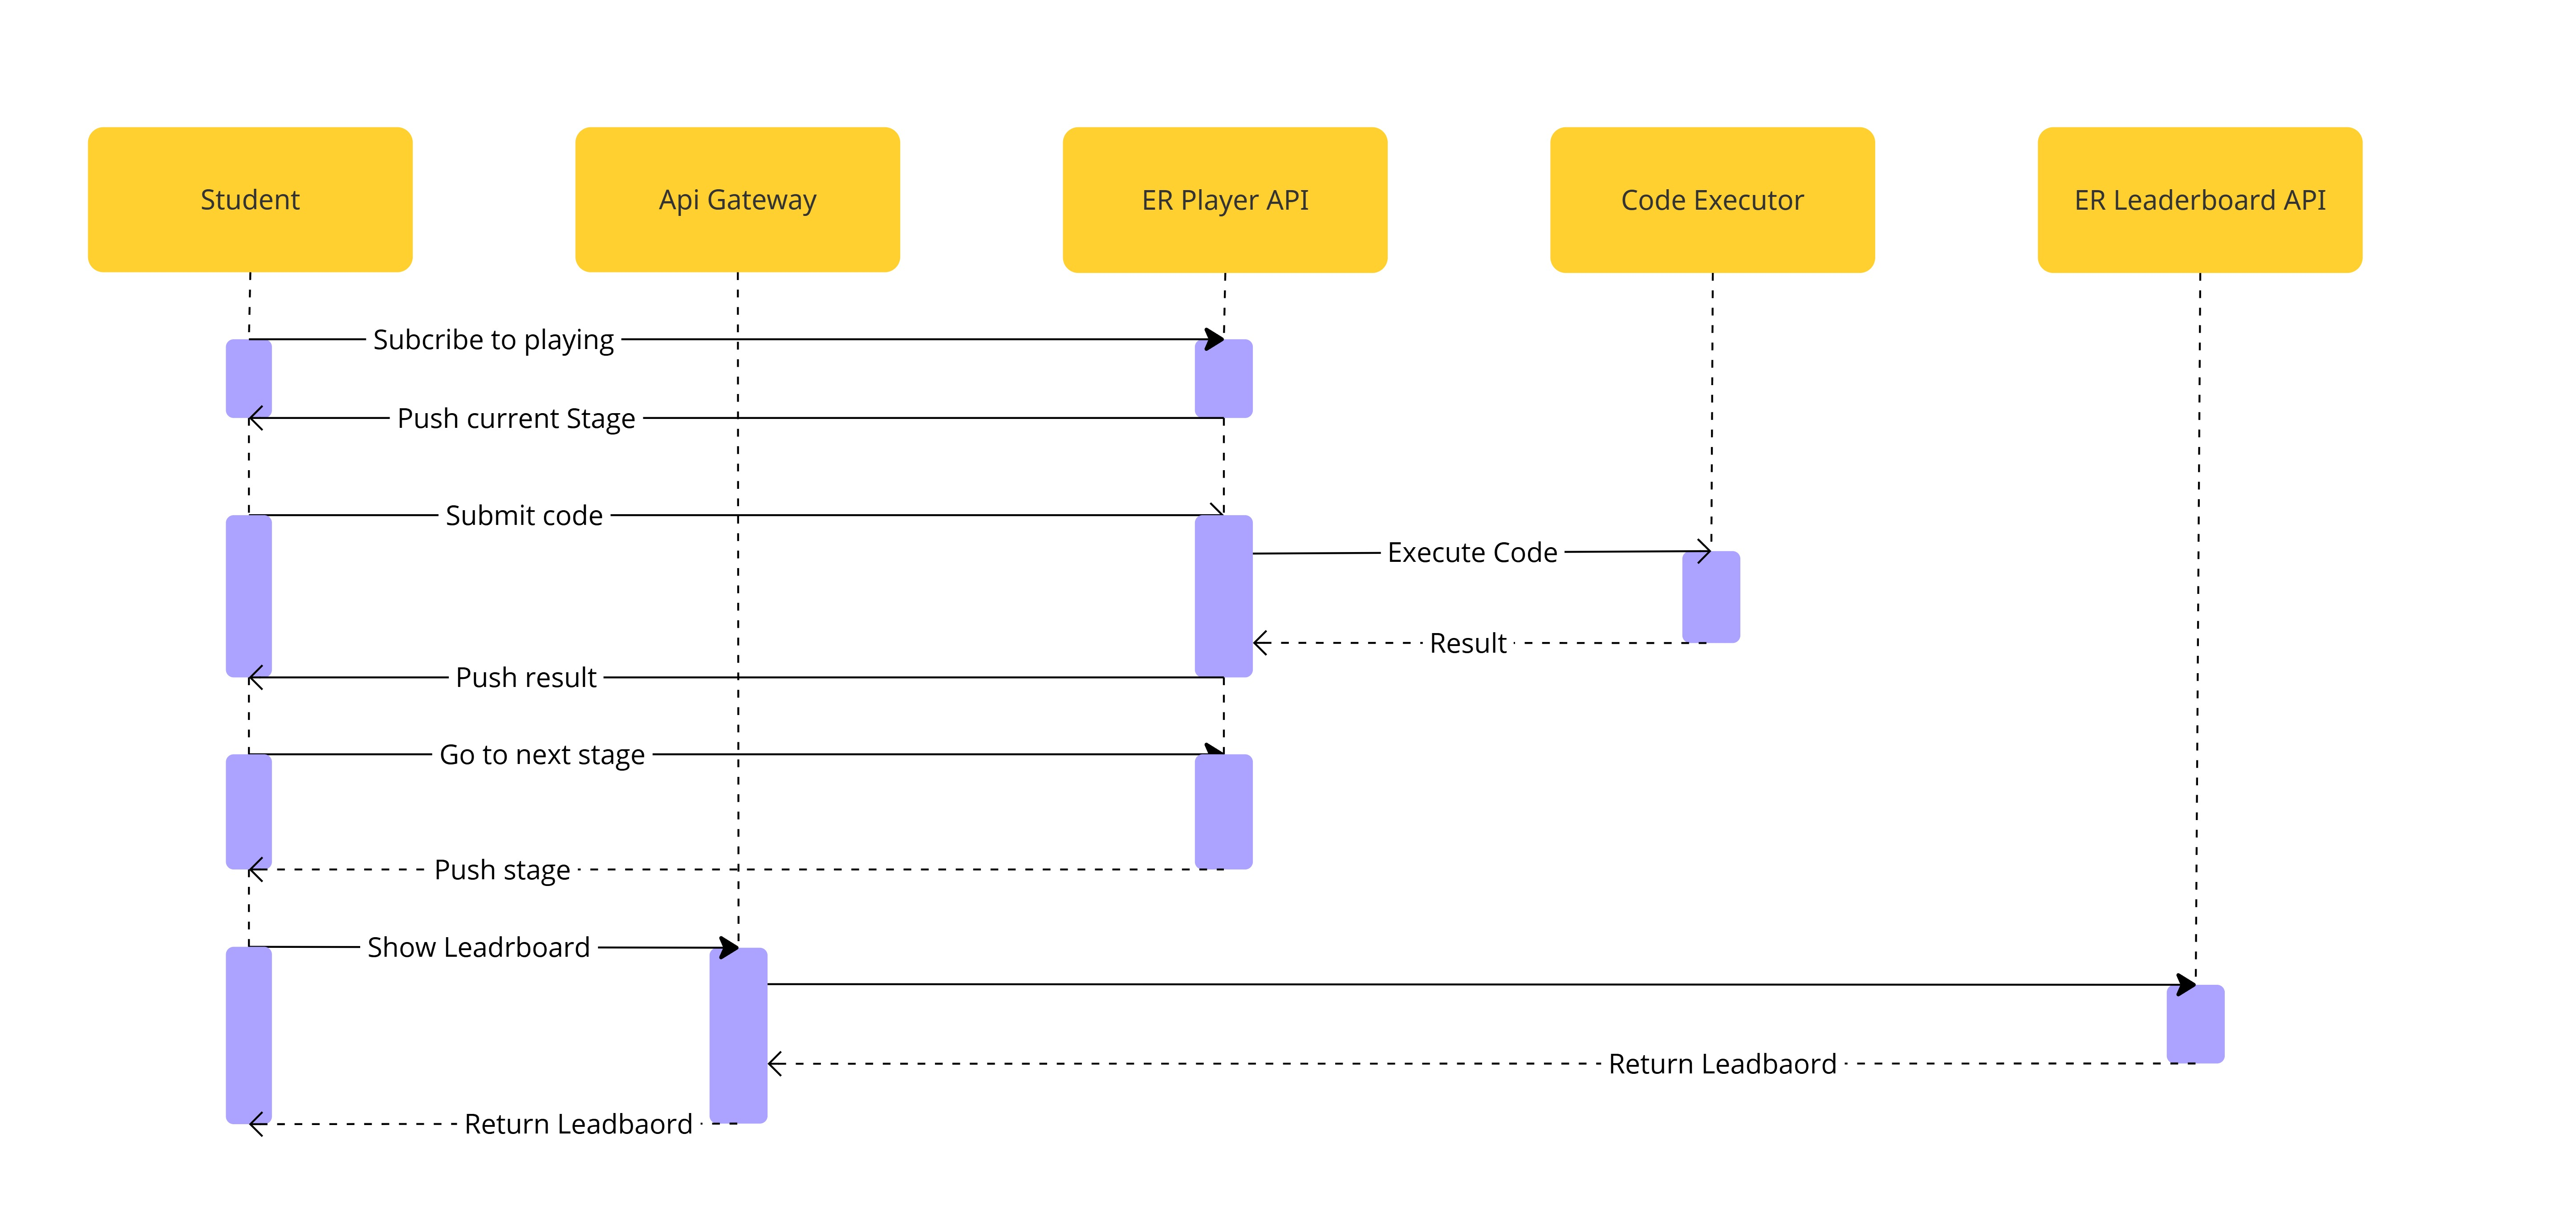
\includegraphics[width=1\linewidth]{images/Sequence Diagrams/SEP1 - EscapeDOOM - Sequenzdiagramm - Play Escaperoom.jpg}
    \caption{Submitting a code solution for a riddle inside an ER}
    \label{fig:sequenceDiag:send_riddle_solution}
\end{figure}